% coming soon


The implementation of the continual planning and switching parts is
based on MAPSIM \cite{brenner:nebel:jaamas09} and is able to use
several planners as the underlying planning system. We use a modified
version of Fast Downward \cite{fast-downward}, which we extended with
the support for actions with success probabilities. Finally, we use
\system{dlib-ml} \cite{king:2009} for successive estimation of the
underlying belief-state.

The baseline approach is using the same continual planning system as
the switching planner, but instead of creating an observation problem
for the decision theoretic planner it will just execute one sensing
action -- assuming that this action will confirm its assumption.

To test our approch we use a robot exploration domain similar to the
one used on a physical robotic system. It involves a robot exploring
an office or living environment and trying to return objects to their
owner.

\begin{figure}[h]
  \centering
  $ Globals
$$ PREFIXES
PREFIX rdf: <http://www.w3.org/1999/02/22-rdf-syntax-ns#>
PREFIX xsd: <http://www.w3.org/2001/XMLSchema#>
PREFIX rdfs: <http://www.w3.org/2000/01/rdf-schema#>
PREFIX owl: <http://www.w3.org/2002/07/owl#>
PREFIX wn: <http://www.dfki.de/cosy/wordnet#>
PREFIX dora: <http://dora.cogx.eu#>

#$ Owlim
#$$ URIS
#file:subarchitectures/coma.sa/ontologies/coma_office.owl
#$$ NAMESPACES
#http://www.dfki.de/cosy/officeenv.owl
#$$ RULES
#/home/kiefer/src/musing/crowl/data/examples/timetest.pie
#MICRO

#$ Pellet
#$$ URIS
#file:subarchitectures/coma.sa/ontologies/coma_office.owl
#$$ NAMESPACES
#http://www.dfki.de/cosy/officeenv.owl
#$$ RULES
#/home/kiefer/src/musing/crowl/data/examples/timetest.pie
#owl-max

$ JenaBase
$$ URIS
file:subarchitectures/coma.sa/ontologies/dora.owl
#file:subarchitectures/coma.sa/ontologies/dora_omics_thingloc.nt
$$ RULES
MICRO
subarchitectures/coma.sa/ontologies/dora.rules
subarchitectures/coma.sa/ontologies/jenaabox.rules
# HUK's abox rules...

#$ JenaRule
#$$ RULES
#subarchitectures/coma.sa/ontologies/coma_office_stripped.rules

  \caption{A exploration domain with three rooms and 13 places. The
    robot is in in the center of room A}
\label{fig:dora2}
\end{figure}
An instance of this domain is shown in figure \ref{fig:dora2}. The
basic building blocks of the domain consist of {\tt rooms}, {\tt
  places} and {\tt objects}. Places are grouped in rooms and objects
(as well as the robot) are always in a place. The robot can move
around the rooms via connections between places given by the {\tt
  connected} predicate. Each room has a (possibly unknown) {\em
  category/} (e.g. kitchen, office, living room) and depending on this
category, objects are placed inside the rooms.

The robot can find out if an object is at a certain place by executing
the {\tt look-for-object} action, which may result in a perception if
the object is in fact there (though some objects are harder to detect
than others -- so absence of a percept is no proof of the object's
absence). Additionally, if the robot is in the presence of a human, it
may simply ask what type of room they are currently in -- but
conducting a dialogue is a bit more costly than simply running the
vision algorithm (cost of 8 vs costs of 3).

We conducted experiments on scenarios of several sizes. The robot's
goal was to find one or more objects and report back their position to
a person. In order to determine the impact of sensor reliability on
both approaches, we also ran tests on identical problems but changed
the sensor model for the goal objects: the probability for percieving
the object if it was there went from 0.9 in the easiest case to 0.65
and 0.4 in the average and hard cases. In addition, we wanted to test
how our system performed on tasks requiring indirect sensing, so we
gave the planner goals to visit a certain type of room (e.g. kitchen
or office). We didn't place any humans in those scenarios, so the only
way of determining the room category was by looking for objects
typical for that room type. As this indirect reasoning is a tasks that
cannot be performed by the continual planner alone, we did not run the
baseline system on those problems.

As the initial state of the problems is stochastic, we ran 50
simulations for each configuration. The samples for the true initial
state were drawn from the same distribution that was used for
planning, so the planner's model matched its simulated world
exactly. Not all problems generated in this manner have a solution. We
did not reject these problems, as we believe that detecting the
non-existance of a solution is important in stochastic domains.


Fast Downward was run with the cyclic causal graph heuristic using A*
search or weighted A* with a weight of 5, depending on the difficulty
of the problem. We then performed multiple tests with different limits
for the belief space size of the decision theoretic subtask. Higher
limits should cause longer planning times but be beneficial to plan
quality as more contingencies can be taken in to account by the POMDP
planner.

Using a satisficing, optimistic serial planner and using continual
planning makes optimising for the expected reward difficult. The
continual planner will in general be overly optimistic regarding the
remaining costs to the goal while being overly pessimistic regarding
the probability of reaching it (as it only regards one trace). This
means that setting the reward function to non-extremal setting had
little effect on the resulting planner behaviour. For this reason, we
chose not to use the expected reward as a metric for our results, as
that information would have been of little value to the
reader. Instead we show the average costs of the plan and the success
rate (as a ratio between solved and solvable problems) separately.

\begin{figure}[h!]
  % \centering
  % 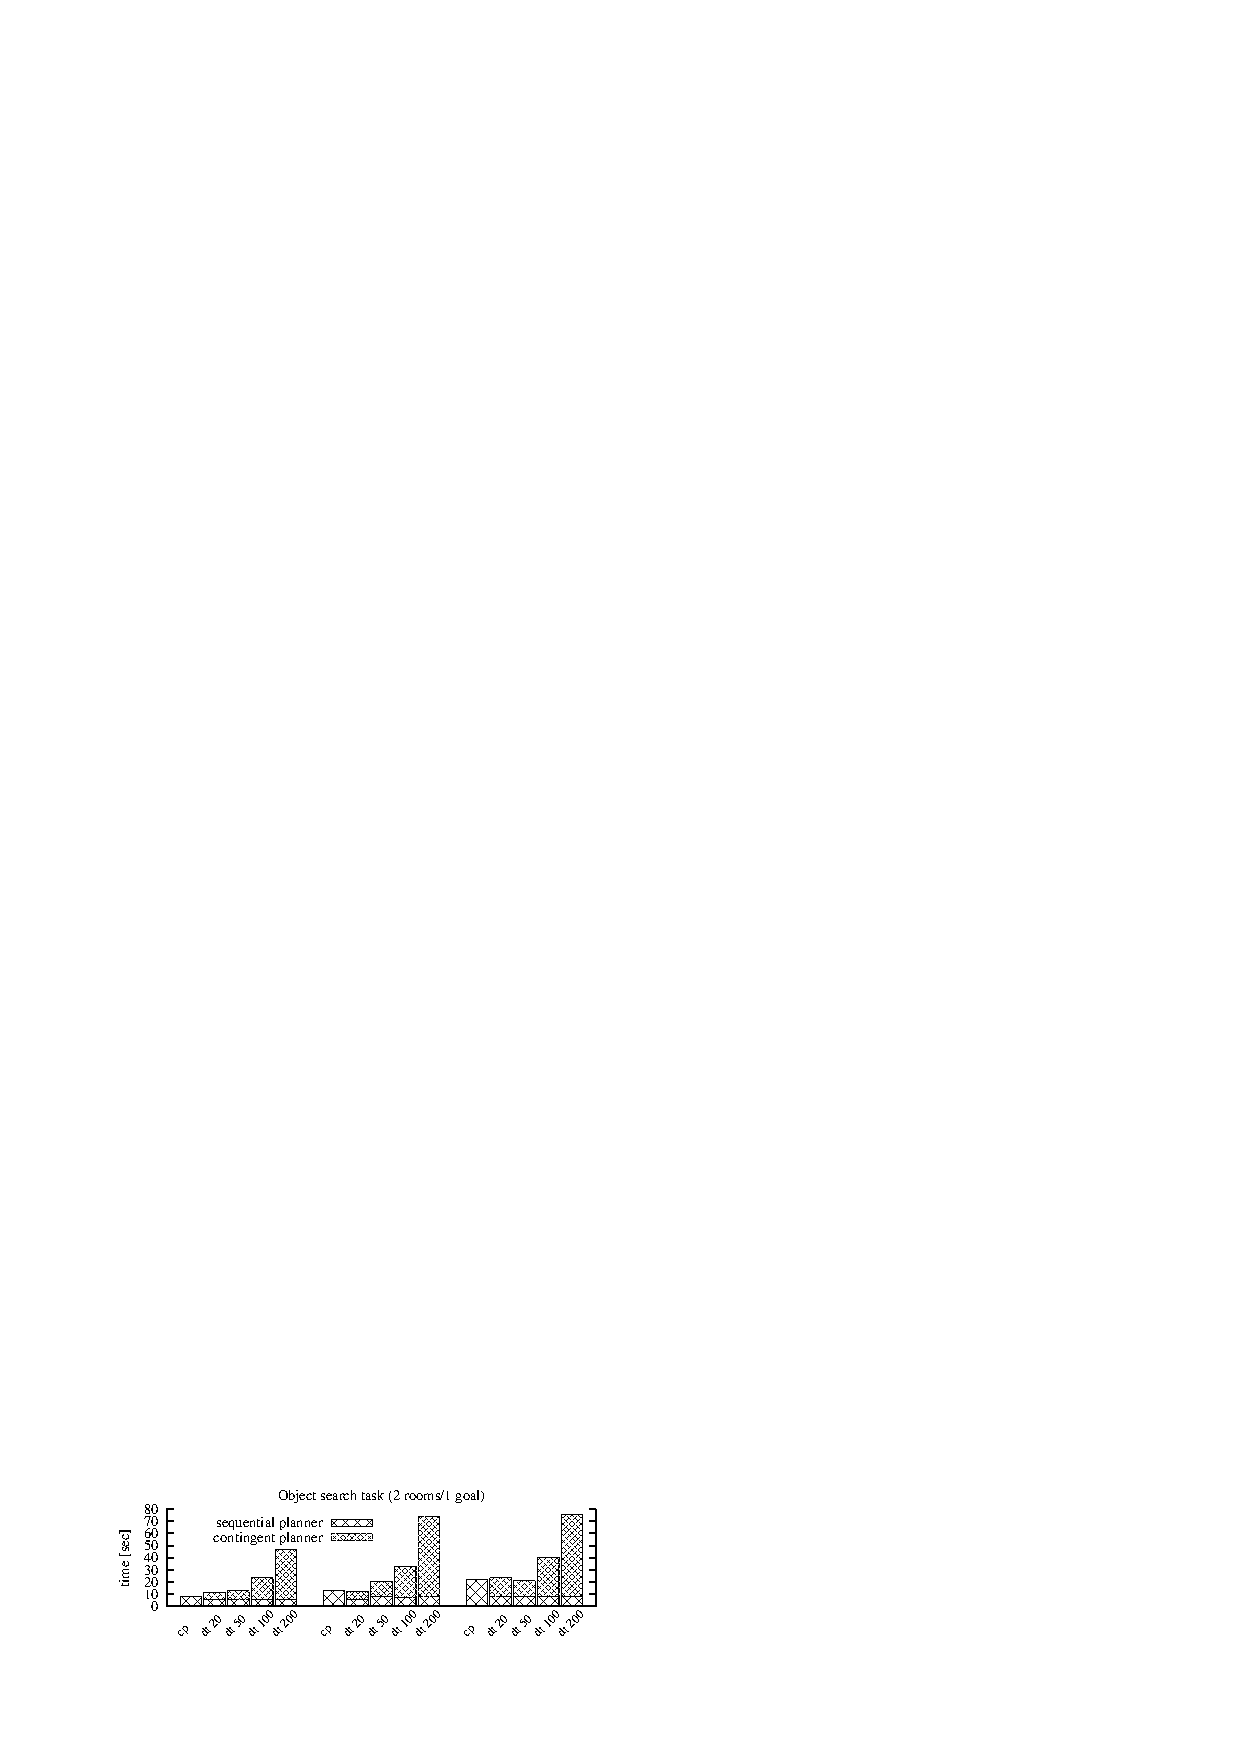
\includegraphics{dora1-time}\hfill
  % \vspace{2mm}
  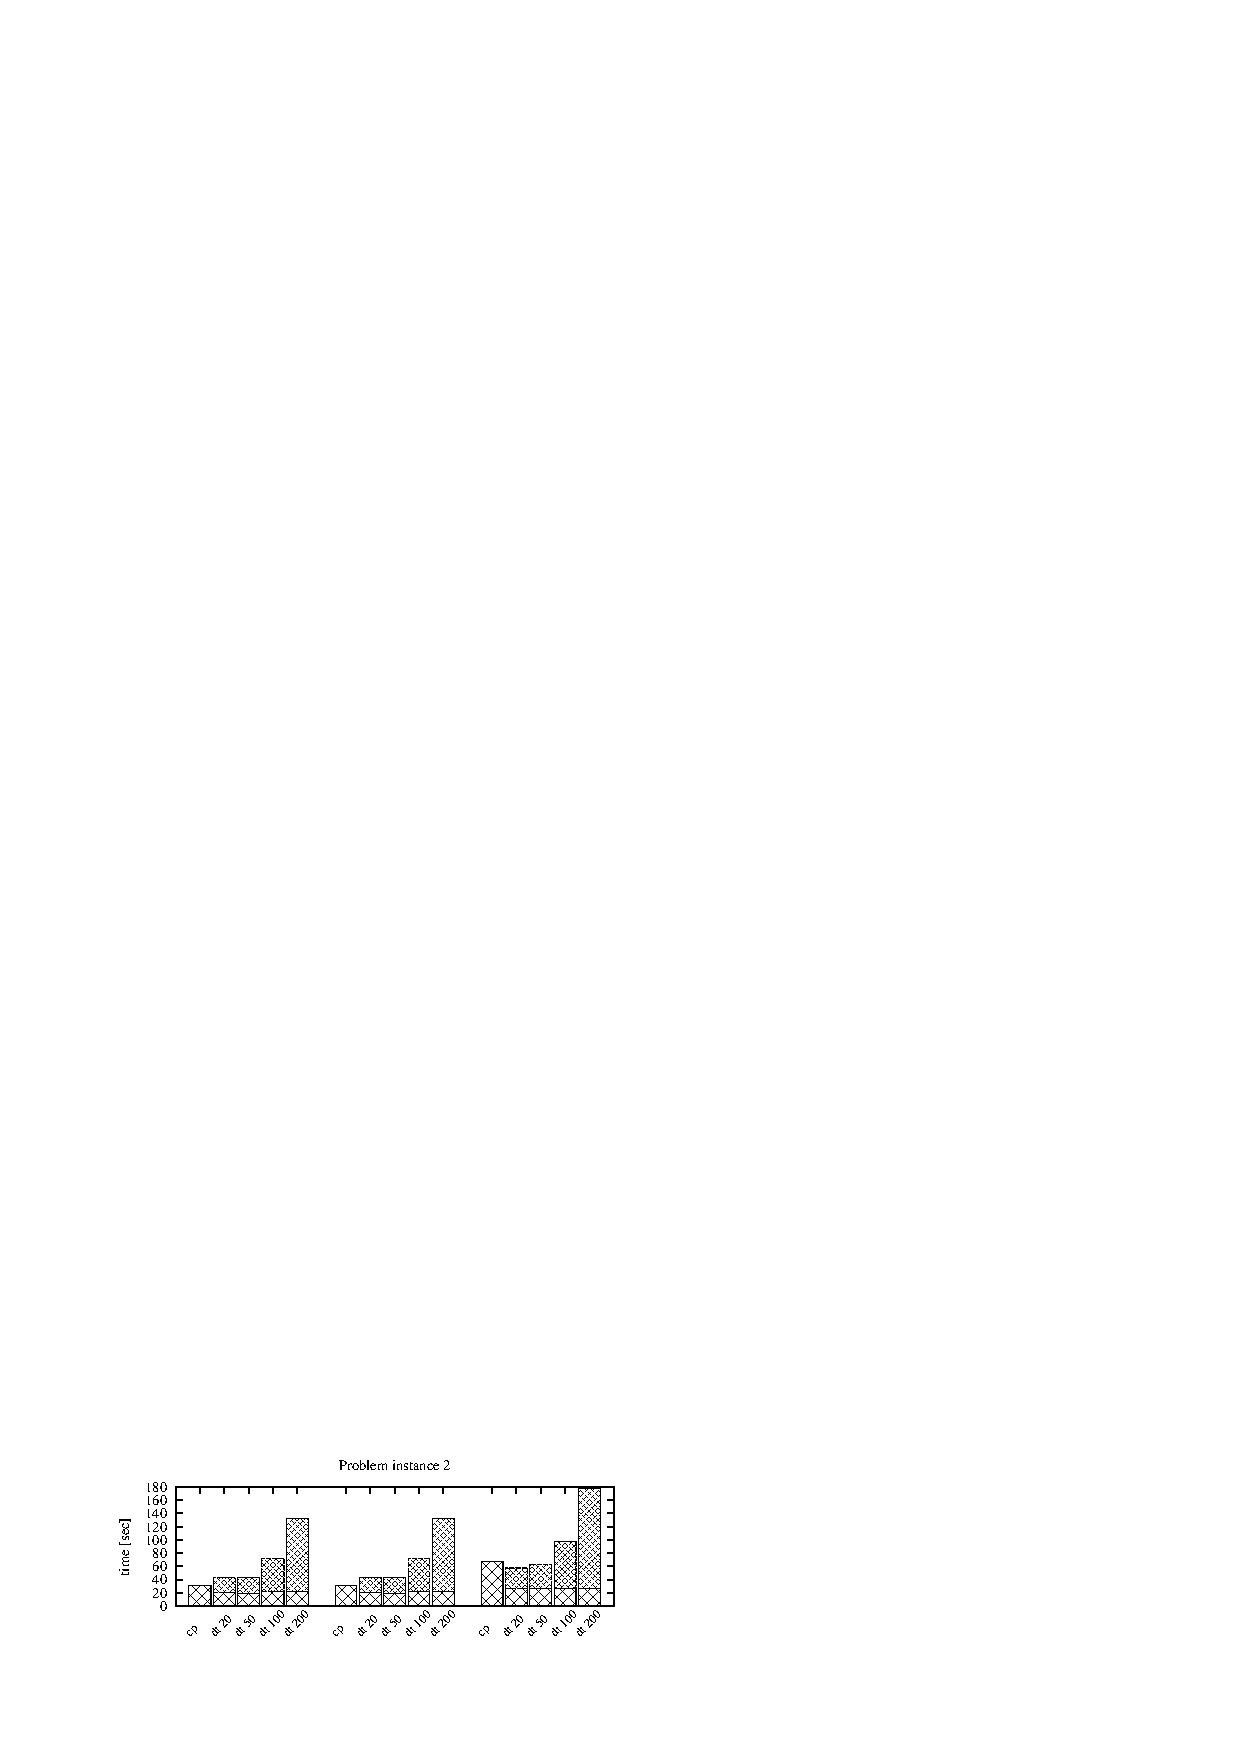
\includegraphics{dora2-time}\hfill
  \vspace{2mm}
  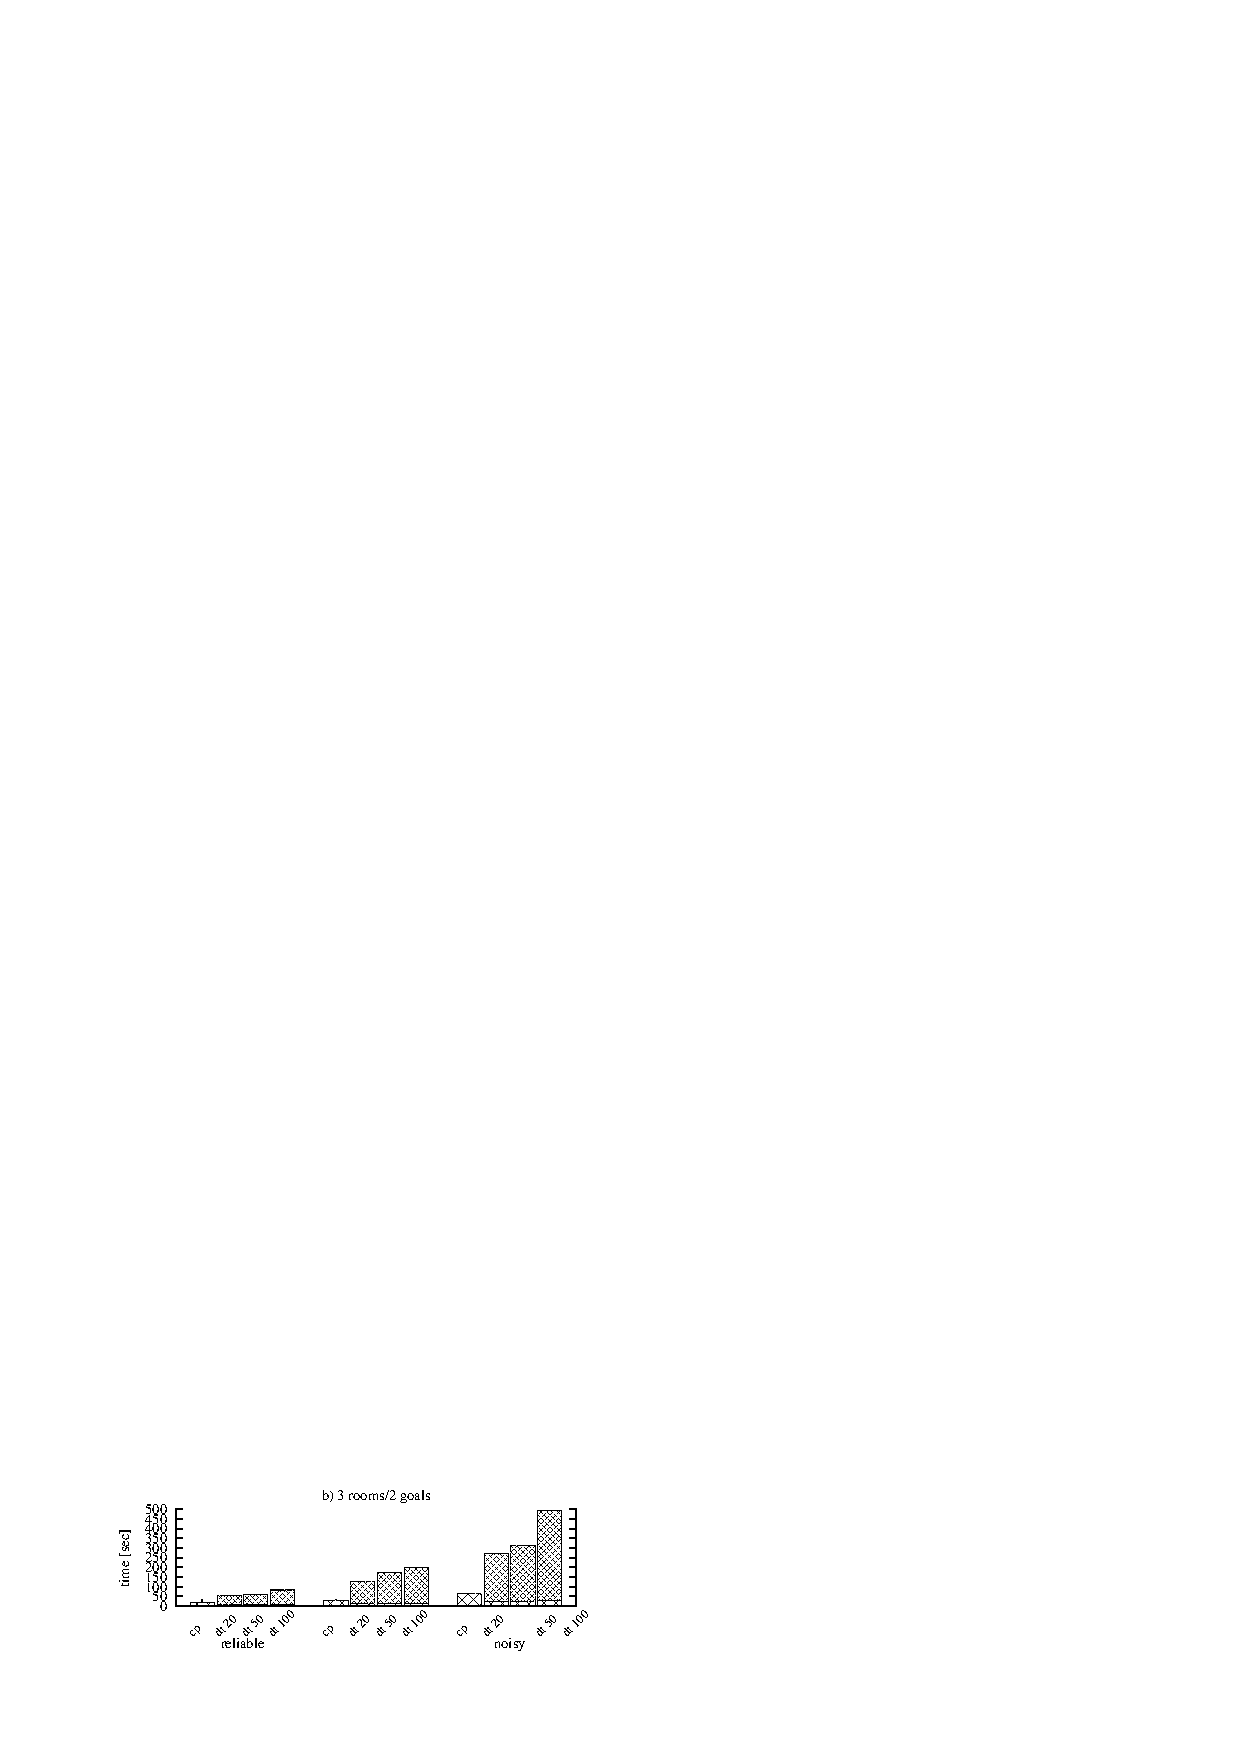
\includegraphics{dora3-time}\hfill
  \vspace{2mm}
  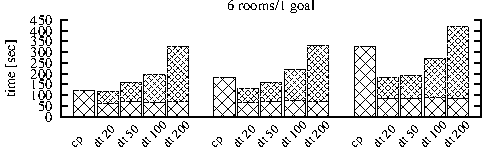
\includegraphics{dora4-time}\hfill
  \vspace{2mm}
  
\includegraphics{dora56-time}\hfill
  \vspace{2mm}
  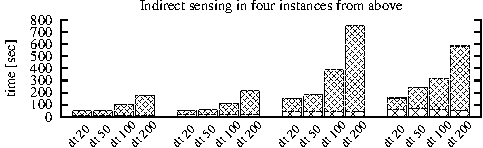
\includegraphics{dora-cat-time}\hfill
  \caption{Average runtime}
  \label{fig:results-time}
\end{figure}

\begin{figure}[h!]
  % \centering
  % 
\includegraphics{dora1-quality}\hfill
  % \vspace{2mm}
  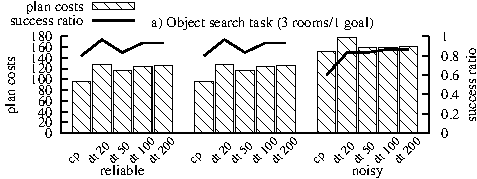
\includegraphics{dora2-quality}\hfill
  \vspace{2mm}
  
\includegraphics{dora3-quality}\hfill
  \vspace{2mm}
  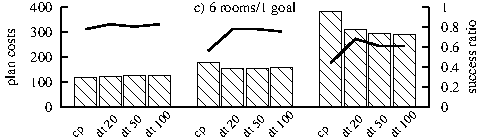
\includegraphics{dora4-quality}\hfill
  \vspace{2mm}
  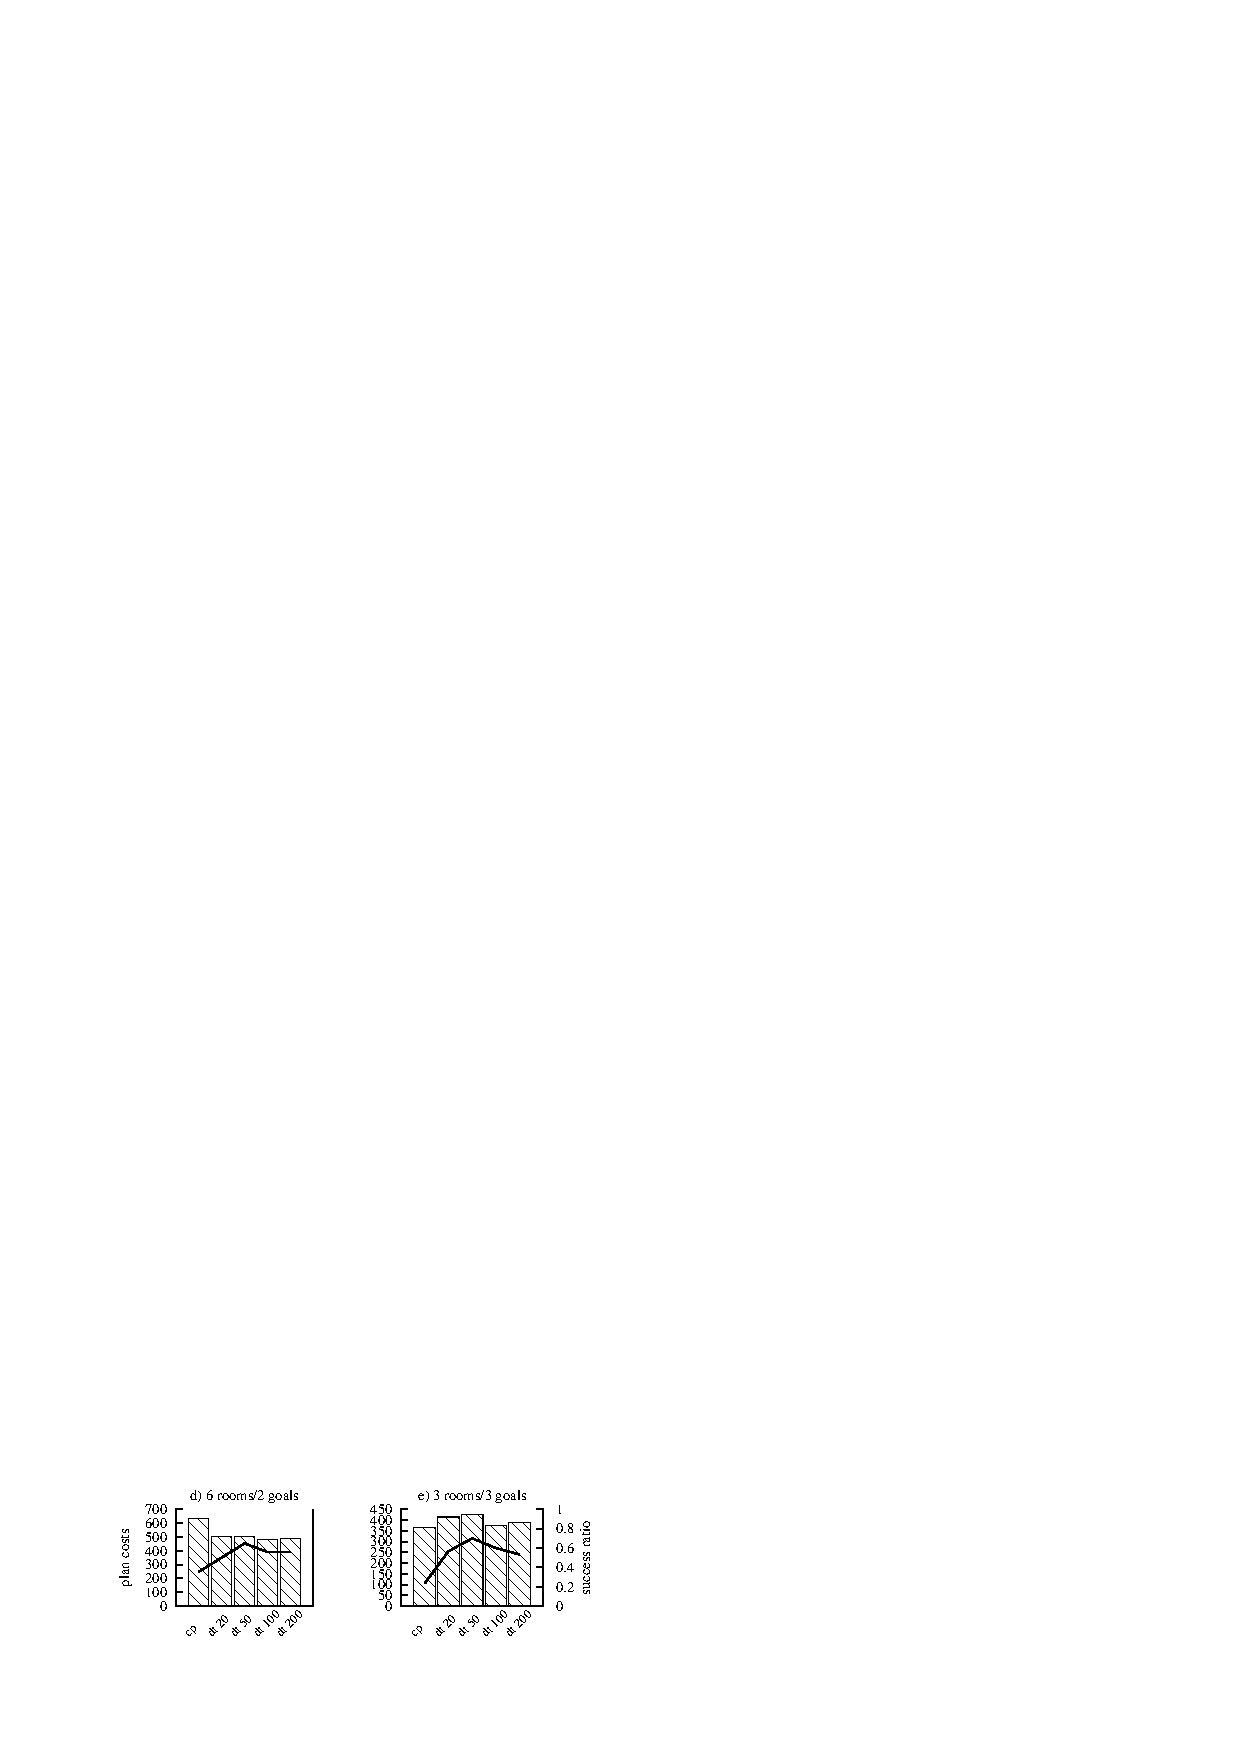
\includegraphics{dora56-quality}\hfill
  \vspace{2mm}
  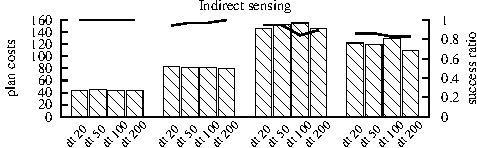
\includegraphics{dora-cat-quality}\hfill
  \caption{Average plan costs and number of successful runs}
  \label{fig:results-quality}
\end{figure}

The graphs in figure \ref{fig:results-time} show the average planning
times. Not surprisingly, the time the POMDP planner takes increases
strongly with larger belief spaces. But for the smaller belief states,
the cost for the decision theoretic planning is compensated by the
decrease of time spent in Fast Downward.

Figure \ref{fig:results-quality} shows the average costs of the
executed plans as well as the percentage of solvable tasks that were
actually solved by the planner. For objects that can be easily
detected there is little gain in using a decision theoretic planner,
as the greedy sensing appoach by the baseline continual planner is
obviously sufficient here. With decreasing sensor reliability the more
sophisticated observation planning pays off: while the resulting plans
are still longer on average, the impact on the number of solved tasks
was much smaller than for the baseline system.

As already mentioned, less aggressive pruning of the initial belief
space resultes in longer runtimes. The impace of the pruning on plan
costs and success rate were limited, though. Increasing the size limit
beyond 50 did rarely pay off because while additional information
might in theroy allow better plans, (add reason here). The indirect
sensing tests show the same result, though with much higher time spent
in the decision theoretic planner. The relatively high success rate
even with small belief spaces might also indicate that the entropy
heuristic for belief space pruning is effective in keeping the most
relevant information.

% We believe that a part of the improvement is due to the segmentation of
% the plan into several subtask, essentially performing hierarchical
% planning. Especially when the continual planner performs badly this is
% a huge gain.

%%% Local Variables: 
%%% mode: latex
%%% TeX-master: "moritz_2011"
%%% End: 
